% Created by tikzDevice version 0.12 on 2018-09-23 23:36:01
% !TEX encoding = UTF-8 Unicode
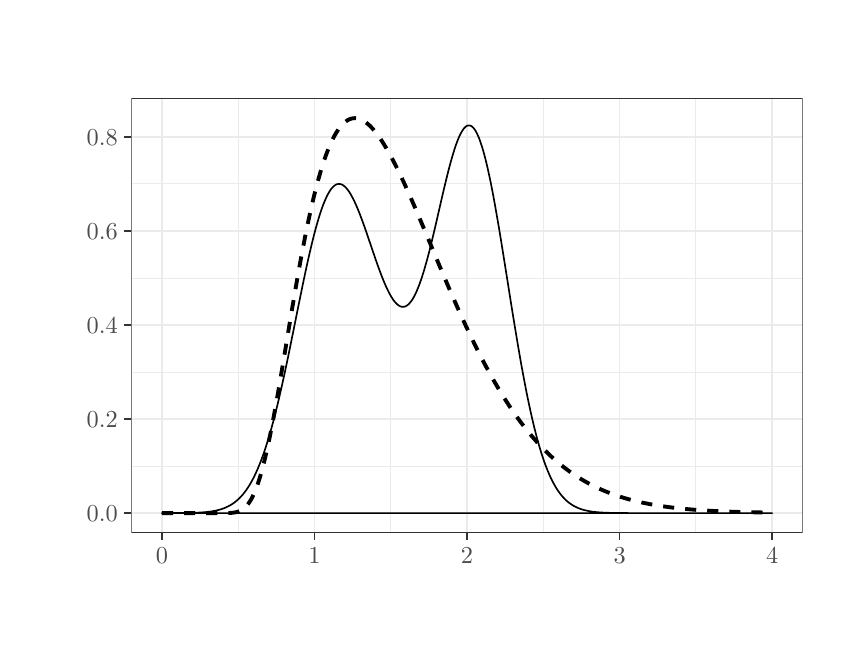
\begin{tikzpicture}[x=1pt,y=1pt]
\definecolor{fillColor}{RGB}{255,255,255}
\path[use as bounding box,fill=fillColor,fill opacity=0.00] (0,0) rectangle (289.08,216.81);
\begin{scope}
\path[clip] (  0.00,  0.00) rectangle (289.08,216.81);
\definecolor{drawColor}{RGB}{255,255,255}
\definecolor{fillColor}{RGB}{255,255,255}

\path[draw=drawColor,line width= 0.6pt,line join=round,line cap=round,fill=fillColor] (  0.00,  0.00) rectangle (289.08,216.81);
\end{scope}
\begin{scope}
\path[clip] ( 37.50, 34.26) rectangle (280.05,191.24);
\definecolor{fillColor}{RGB}{255,255,255}

\path[fill=fillColor] ( 37.50, 34.26) rectangle (280.05,191.24);
\definecolor{drawColor}{gray}{0.92}

\path[draw=drawColor,line width= 0.3pt,line join=round] ( 37.50, 58.39) --
	(280.05, 58.39);

\path[draw=drawColor,line width= 0.3pt,line join=round] ( 37.50, 92.38) --
	(280.05, 92.38);

\path[draw=drawColor,line width= 0.3pt,line join=round] ( 37.50,126.37) --
	(280.05,126.37);

\path[draw=drawColor,line width= 0.3pt,line join=round] ( 37.50,160.36) --
	(280.05,160.36);

\path[draw=drawColor,line width= 0.3pt,line join=round] ( 76.08, 34.26) --
	( 76.08,191.24);

\path[draw=drawColor,line width= 0.3pt,line join=round] (131.21, 34.26) --
	(131.21,191.24);

\path[draw=drawColor,line width= 0.3pt,line join=round] (186.33, 34.26) --
	(186.33,191.24);

\path[draw=drawColor,line width= 0.3pt,line join=round] (241.46, 34.26) --
	(241.46,191.24);

\path[draw=drawColor,line width= 0.6pt,line join=round] ( 37.50, 41.39) --
	(280.05, 41.39);

\path[draw=drawColor,line width= 0.6pt,line join=round] ( 37.50, 75.38) --
	(280.05, 75.38);

\path[draw=drawColor,line width= 0.6pt,line join=round] ( 37.50,109.37) --
	(280.05,109.37);

\path[draw=drawColor,line width= 0.6pt,line join=round] ( 37.50,143.37) --
	(280.05,143.37);

\path[draw=drawColor,line width= 0.6pt,line join=round] ( 37.50,177.36) --
	(280.05,177.36);

\path[draw=drawColor,line width= 0.6pt,line join=round] ( 48.52, 34.26) --
	( 48.52,191.24);

\path[draw=drawColor,line width= 0.6pt,line join=round] (103.65, 34.26) --
	(103.65,191.24);

\path[draw=drawColor,line width= 0.6pt,line join=round] (158.77, 34.26) --
	(158.77,191.24);

\path[draw=drawColor,line width= 0.6pt,line join=round] (213.90, 34.26) --
	(213.90,191.24);

\path[draw=drawColor,line width= 0.6pt,line join=round] (269.02, 34.26) --
	(269.02,191.24);
\definecolor{drawColor}{RGB}{0,0,0}

\path[draw=drawColor,line width= 0.6pt,line join=round,line cap=round] ( 48.52, 41.40) --
	( 48.95, 41.40) --
	( 49.38, 41.40) --
	( 49.82, 41.40) --
	( 50.25, 41.40) --
	( 50.68, 41.40) --
	( 51.11, 41.40) --
	( 51.54, 41.40) --
	( 51.97, 41.40) --
	( 52.40, 41.41) --
	( 52.84, 41.41) --
	( 53.27, 41.41) --
	( 53.70, 41.41) --
	( 54.13, 41.41) --
	( 54.56, 41.42) --
	( 54.99, 41.42) --
	( 55.42, 41.42) --
	( 55.86, 41.43) --
	( 56.29, 41.43) --
	( 56.72, 41.44) --
	( 57.15, 41.44) --
	( 57.58, 41.45) --
	( 58.01, 41.46) --
	( 58.45, 41.47) --
	( 58.88, 41.48) --
	( 59.31, 41.49) --
	( 59.74, 41.50) --
	( 60.17, 41.51) --
	( 60.60, 41.53) --
	( 61.03, 41.55) --
	( 61.47, 41.57) --
	( 61.90, 41.59) --
	( 62.33, 41.61) --
	( 62.76, 41.64) --
	( 63.19, 41.67) --
	( 63.62, 41.70) --
	( 64.05, 41.74) --
	( 64.49, 41.78) --
	( 64.92, 41.82) --
	( 65.35, 41.87) --
	( 65.78, 41.93) --
	( 66.21, 41.99) --
	( 66.64, 42.05) --
	( 67.08, 42.13) --
	( 67.51, 42.21) --
	( 67.94, 42.29) --
	( 68.37, 42.39) --
	( 68.80, 42.49) --
	( 69.23, 42.61) --
	( 69.66, 42.73) --
	( 70.10, 42.87) --
	( 70.53, 43.01) --
	( 70.96, 43.17) --
	( 71.39, 43.35) --
	( 71.82, 43.53) --
	( 72.25, 43.74) --
	( 72.68, 43.96) --
	( 73.12, 44.19) --
	( 73.55, 44.45) --
	( 73.98, 44.72) --
	( 74.41, 45.02) --
	( 74.84, 45.33) --
	( 75.27, 45.68) --
	( 75.71, 46.04) --
	( 76.14, 46.43) --
	( 76.57, 46.85) --
	( 77.00, 47.30) --
	( 77.43, 47.76) --
	( 77.86, 48.27) --
	( 78.29, 48.81) --
	( 78.73, 49.38) --
	( 79.16, 49.99) --
	( 79.59, 50.63) --
	( 80.02, 51.31) --
	( 80.45, 52.02) --
	( 80.88, 52.79) --
	( 81.32, 53.58) --
	( 81.75, 54.41) --
	( 82.18, 55.30) --
	( 82.61, 56.23) --
	( 83.04, 57.19) --
	( 83.47, 58.22) --
	( 83.90, 59.29) --
	( 84.34, 60.39) --
	( 84.77, 61.55) --
	( 85.20, 62.76) --
	( 85.63, 64.01) --
	( 86.06, 65.32) --
	( 86.49, 66.68) --
	( 86.92, 68.08) --
	( 87.36, 69.52) --
	( 87.79, 71.03) --
	( 88.22, 72.58) --
	( 88.65, 74.17) --
	( 89.08, 75.82) --
	( 89.51, 77.51) --
	( 89.95, 79.24) --
	( 90.38, 81.01) --
	( 90.81, 82.84) --
	( 91.24, 84.69) --
	( 91.67, 86.58) --
	( 92.10, 88.52) --
	( 92.53, 90.48) --
	( 92.97, 92.48) --
	( 93.40, 94.51) --
	( 93.83, 96.56) --
	( 94.26, 98.63) --
	( 94.69,100.73) --
	( 95.12,102.84) --
	( 95.55,104.97) --
	( 95.99,107.10) --
	( 96.42,109.25) --
	( 96.85,111.39) --
	( 97.28,113.54) --
	( 97.71,115.68) --
	( 98.14,117.81) --
	( 98.58,119.94) --
	( 99.01,122.04) --
	( 99.44,124.13) --
	( 99.87,126.19) --
	(100.30,128.22) --
	(100.73,130.22) --
	(101.16,132.19) --
	(101.60,134.11) --
	(102.03,135.98) --
	(102.46,137.82) --
	(102.89,139.60) --
	(103.32,141.32) --
	(103.75,142.99) --
	(104.19,144.61) --
	(104.62,146.13) --
	(105.05,147.61) --
	(105.48,149.02) --
	(105.91,150.34) --
	(106.34,151.59) --
	(106.77,152.77) --
	(107.21,153.86) --
	(107.64,154.87) --
	(108.07,155.81) --
	(108.50,156.65) --
	(108.93,157.40) --
	(109.36,158.08) --
	(109.79,158.68) --
	(110.23,159.16) --
	(110.66,159.57) --
	(111.09,159.91) --
	(111.52,160.13) --
	(111.95,160.28) --
	(112.38,160.36) --
	(112.82,160.33) --
	(113.25,160.22) --
	(113.68,160.04) --
	(114.11,159.78) --
	(114.54,159.43) --
	(114.97,159.02) --
	(115.40,158.53) --
	(115.84,157.96) --
	(116.27,157.33) --
	(116.70,156.65) --
	(117.13,155.87) --
	(117.56,155.05) --
	(117.99,154.19) --
	(118.42,153.26) --
	(118.86,152.28) --
	(119.29,151.26) --
	(119.72,150.20) --
	(120.15,149.09) --
	(120.58,147.95) --
	(121.01,146.79) --
	(121.45,145.59) --
	(121.88,144.37) --
	(122.31,143.13) --
	(122.74,141.88) --
	(123.17,140.61) --
	(123.60,139.34) --
	(124.03,138.07) --
	(124.47,136.79) --
	(124.90,135.52) --
	(125.33,134.26) --
	(125.76,133.01) --
	(126.19,131.78) --
	(126.62,130.56) --
	(127.05,129.38) --
	(127.49,128.22) --
	(127.92,127.08) --
	(128.35,125.99) --
	(128.78,124.94) --
	(129.21,123.92) --
	(129.64,122.96) --
	(130.08,122.04) --
	(130.51,121.17) --
	(130.94,120.36) --
	(131.37,119.62) --
	(131.80,118.93) --
	(132.23,118.29) --
	(132.66,117.75) --
	(133.10,117.26) --
	(133.53,116.83) --
	(133.96,116.50) --
	(134.39,116.24) --
	(134.82,116.04) --
	(135.25,115.94) --
	(135.69,115.93) --
	(136.12,115.98) --
	(136.55,116.12) --
	(136.98,116.36) --
	(137.41,116.67) --
	(137.84,117.06) --
	(138.27,117.57) --
	(138.71,118.14) --
	(139.14,118.78) --
	(139.57,119.55) --
	(140.00,120.38) --
	(140.43,121.28) --
	(140.86,122.29) --
	(141.29,123.37) --
	(141.73,124.52) --
	(142.16,125.75) --
	(142.59,127.06) --
	(143.02,128.43) --
	(143.45,129.86) --
	(143.88,131.38) --
	(144.32,132.94) --
	(144.75,134.55) --
	(145.18,136.23) --
	(145.61,137.94) --
	(146.04,139.69) --
	(146.47,141.49) --
	(146.90,143.31) --
	(147.34,145.15) --
	(147.77,147.02) --
	(148.20,148.90) --
	(148.63,150.78) --
	(149.06,152.67) --
	(149.49,154.54) --
	(149.92,156.41) --
	(150.36,158.26) --
	(150.79,160.07) --
	(151.22,161.86) --
	(151.65,163.61) --
	(152.08,165.31) --
	(152.51,166.95) --
	(152.95,168.55) --
	(153.38,170.07) --
	(153.81,171.51) --
	(154.24,172.89) --
	(154.67,174.19) --
	(155.10,175.38) --
	(155.53,176.49) --
	(155.97,177.52) --
	(156.40,178.40) --
	(156.83,179.19) --
	(157.26,179.89) --
	(157.69,180.45) --
	(158.12,180.89) --
	(158.56,181.23) --
	(158.99,181.43) --
	(159.42,181.49) --
	(159.85,181.44) --
	(160.28,181.27) --
	(160.71,180.94) --
	(161.14,180.50) --
	(161.58,179.95) --
	(162.01,179.22) --
	(162.44,178.38) --
	(162.87,177.45) --
	(163.30,176.35) --
	(163.73,175.13) --
	(164.16,173.82) --
	(164.60,172.37) --
	(165.03,170.80) --
	(165.46,169.14) --
	(165.89,167.38) --
	(166.32,165.49) --
	(166.75,163.52) --
	(167.19,161.48) --
	(167.62,159.32) --
	(168.05,157.09) --
	(168.48,154.80) --
	(168.91,152.42) --
	(169.34,149.99) --
	(169.77,147.51) --
	(170.21,144.97) --
	(170.64,142.38) --
	(171.07,139.76) --
	(171.50,137.11) --
	(171.93,134.42) --
	(172.36,131.72) --
	(172.79,129.01) --
	(173.23,126.29) --
	(173.66,123.56) --
	(174.09,120.84) --
	(174.52,118.13) --
	(174.95,115.43) --
	(175.38,112.75) --
	(175.82,110.09) --
	(176.25,107.47) --
	(176.68,104.87) --
	(177.11,102.31) --
	(177.54, 99.80) --
	(177.97, 97.32) --
	(178.40, 94.89) --
	(178.84, 92.52) --
	(179.27, 90.20) --
	(179.70, 87.92) --
	(180.13, 85.72) --
	(180.56, 83.57) --
	(180.99, 81.47) --
	(181.43, 79.45) --
	(181.86, 77.49) --
	(182.29, 75.58) --
	(182.72, 73.74) --
	(183.15, 71.98) --
	(183.58, 70.28) --
	(184.01, 68.62) --
	(184.45, 67.06) --
	(184.88, 65.55) --
	(185.31, 64.10) --
	(185.74, 62.72) --
	(186.17, 61.41) --
	(186.60, 60.14) --
	(187.03, 58.94) --
	(187.47, 57.81) --
	(187.90, 56.72) --
	(188.33, 55.69) --
	(188.76, 54.72) --
	(189.19, 53.80) --
	(189.62, 52.92) --
	(190.06, 52.11) --
	(190.49, 51.34) --
	(190.92, 50.60) --
	(191.35, 49.92) --
	(191.78, 49.28) --
	(192.21, 48.68) --
	(192.64, 48.11) --
	(193.08, 47.59) --
	(193.51, 47.10) --
	(193.94, 46.64) --
	(194.37, 46.21) --
	(194.80, 45.82) --
	(195.23, 45.44) --
	(195.66, 45.10) --
	(196.10, 44.79) --
	(196.53, 44.49) --
	(196.96, 44.22) --
	(197.39, 43.97) --
	(197.82, 43.74) --
	(198.25, 43.53) --
	(198.69, 43.33) --
	(199.12, 43.15) --
	(199.55, 42.99) --
	(199.98, 42.84) --
	(200.41, 42.70) --
	(200.84, 42.57) --
	(201.27, 42.46) --
	(201.71, 42.35) --
	(202.14, 42.26) --
	(202.57, 42.17) --
	(203.00, 42.09) --
	(203.43, 42.02) --
	(203.86, 41.95) --
	(204.29, 41.90) --
	(204.73, 41.84) --
	(205.16, 41.79) --
	(205.59, 41.75) --
	(206.02, 41.71) --
	(206.45, 41.68) --
	(206.88, 41.65) --
	(207.32, 41.62) --
	(207.75, 41.59) --
	(208.18, 41.57) --
	(208.61, 41.55) --
	(209.04, 41.53) --
	(209.47, 41.52) --
	(209.90, 41.50) --
	(210.34, 41.49) --
	(210.77, 41.48) --
	(211.20, 41.47) --
	(211.63, 41.46) --
	(212.06, 41.45) --
	(212.49, 41.44) --
	(212.93, 41.44) --
	(213.36, 41.43) --
	(213.79, 41.43) --
	(214.22, 41.42) --
	(214.65, 41.42) --
	(215.08, 41.42) --
	(215.51, 41.41) --
	(215.95, 41.41) --
	(216.38, 41.41) --
	(216.81, 41.41) --
	(217.24, 41.40) --
	(217.67, 41.40) --
	(218.10, 41.40) --
	(218.53, 41.40) --
	(218.97, 41.40) --
	(219.40, 41.40) --
	(219.83, 41.40) --
	(220.26, 41.40) --
	(220.69, 41.40) --
	(221.12, 41.40) --
	(221.56, 41.40) --
	(221.99, 41.40) --
	(222.42, 41.40) --
	(222.85, 41.40) --
	(223.28, 41.40) --
	(223.71, 41.40) --
	(224.14, 41.39) --
	(224.58, 41.39) --
	(225.01, 41.39) --
	(225.44, 41.39) --
	(225.87, 41.39) --
	(226.30, 41.39) --
	(226.73, 41.39) --
	(227.16, 41.39) --
	(227.60, 41.39) --
	(228.03, 41.39) --
	(228.46, 41.39) --
	(228.89, 41.39) --
	(229.32, 41.39) --
	(229.75, 41.39) --
	(230.19, 41.39) --
	(230.62, 41.39) --
	(231.05, 41.39) --
	(231.48, 41.39) --
	(231.91, 41.39) --
	(232.34, 41.39) --
	(232.77, 41.39) --
	(233.21, 41.39) --
	(233.64, 41.39) --
	(234.07, 41.39) --
	(234.50, 41.39) --
	(234.93, 41.39) --
	(235.36, 41.39) --
	(235.80, 41.39) --
	(236.23, 41.39) --
	(236.66, 41.39) --
	(237.09, 41.39) --
	(237.52, 41.39) --
	(237.95, 41.39) --
	(238.38, 41.39) --
	(238.82, 41.39) --
	(239.25, 41.39) --
	(239.68, 41.39) --
	(240.11, 41.39) --
	(240.54, 41.39) --
	(240.97, 41.39) --
	(241.40, 41.39) --
	(241.84, 41.39) --
	(242.27, 41.39) --
	(242.70, 41.39) --
	(243.13, 41.39) --
	(243.56, 41.39) --
	(243.99, 41.39) --
	(244.43, 41.39) --
	(244.86, 41.39) --
	(245.29, 41.39) --
	(245.72, 41.39) --
	(246.15, 41.39) --
	(246.58, 41.39) --
	(247.01, 41.39) --
	(247.45, 41.39) --
	(247.88, 41.39) --
	(248.31, 41.39) --
	(248.74, 41.39) --
	(249.17, 41.39) --
	(249.60, 41.39) --
	(250.03, 41.39) --
	(250.47, 41.39) --
	(250.90, 41.39) --
	(251.33, 41.39) --
	(251.76, 41.39) --
	(252.19, 41.39) --
	(252.62, 41.39) --
	(253.06, 41.39) --
	(253.49, 41.39) --
	(253.92, 41.39) --
	(254.35, 41.39) --
	(254.78, 41.39) --
	(255.21, 41.39) --
	(255.64, 41.39) --
	(256.08, 41.39) --
	(256.51, 41.39) --
	(256.94, 41.39) --
	(257.37, 41.39) --
	(257.80, 41.39) --
	(258.23, 41.39) --
	(258.67, 41.39) --
	(259.10, 41.39) --
	(259.53, 41.39) --
	(259.96, 41.39) --
	(260.39, 41.39) --
	(260.82, 41.39) --
	(261.25, 41.39) --
	(261.69, 41.39) --
	(262.12, 41.39) --
	(262.55, 41.39) --
	(262.98, 41.39) --
	(263.41, 41.39) --
	(263.84, 41.39) --
	(264.27, 41.39) --
	(264.71, 41.39) --
	(265.14, 41.39) --
	(265.57, 41.39) --
	(266.00, 41.39) --
	(266.43, 41.39) --
	(266.86, 41.39) --
	(267.30, 41.39) --
	(267.73, 41.39) --
	(268.16, 41.39) --
	(268.59, 41.39) --
	(269.02, 41.39) --
	(269.02, 41.39) --
	(268.59, 41.39) --
	(268.16, 41.39) --
	(267.73, 41.39) --
	(267.30, 41.39) --
	(266.86, 41.39) --
	(266.43, 41.39) --
	(266.00, 41.39) --
	(265.57, 41.39) --
	(265.14, 41.39) --
	(264.71, 41.39) --
	(264.27, 41.39) --
	(263.84, 41.39) --
	(263.41, 41.39) --
	(262.98, 41.39) --
	(262.55, 41.39) --
	(262.12, 41.39) --
	(261.69, 41.39) --
	(261.25, 41.39) --
	(260.82, 41.39) --
	(260.39, 41.39) --
	(259.96, 41.39) --
	(259.53, 41.39) --
	(259.10, 41.39) --
	(258.67, 41.39) --
	(258.23, 41.39) --
	(257.80, 41.39) --
	(257.37, 41.39) --
	(256.94, 41.39) --
	(256.51, 41.39) --
	(256.08, 41.39) --
	(255.64, 41.39) --
	(255.21, 41.39) --
	(254.78, 41.39) --
	(254.35, 41.39) --
	(253.92, 41.39) --
	(253.49, 41.39) --
	(253.06, 41.39) --
	(252.62, 41.39) --
	(252.19, 41.39) --
	(251.76, 41.39) --
	(251.33, 41.39) --
	(250.90, 41.39) --
	(250.47, 41.39) --
	(250.03, 41.39) --
	(249.60, 41.39) --
	(249.17, 41.39) --
	(248.74, 41.39) --
	(248.31, 41.39) --
	(247.88, 41.39) --
	(247.45, 41.39) --
	(247.01, 41.39) --
	(246.58, 41.39) --
	(246.15, 41.39) --
	(245.72, 41.39) --
	(245.29, 41.39) --
	(244.86, 41.39) --
	(244.43, 41.39) --
	(243.99, 41.39) --
	(243.56, 41.39) --
	(243.13, 41.39) --
	(242.70, 41.39) --
	(242.27, 41.39) --
	(241.84, 41.39) --
	(241.40, 41.39) --
	(240.97, 41.39) --
	(240.54, 41.39) --
	(240.11, 41.39) --
	(239.68, 41.39) --
	(239.25, 41.39) --
	(238.82, 41.39) --
	(238.38, 41.39) --
	(237.95, 41.39) --
	(237.52, 41.39) --
	(237.09, 41.39) --
	(236.66, 41.39) --
	(236.23, 41.39) --
	(235.80, 41.39) --
	(235.36, 41.39) --
	(234.93, 41.39) --
	(234.50, 41.39) --
	(234.07, 41.39) --
	(233.64, 41.39) --
	(233.21, 41.39) --
	(232.77, 41.39) --
	(232.34, 41.39) --
	(231.91, 41.39) --
	(231.48, 41.39) --
	(231.05, 41.39) --
	(230.62, 41.39) --
	(230.19, 41.39) --
	(229.75, 41.39) --
	(229.32, 41.39) --
	(228.89, 41.39) --
	(228.46, 41.39) --
	(228.03, 41.39) --
	(227.60, 41.39) --
	(227.16, 41.39) --
	(226.73, 41.39) --
	(226.30, 41.39) --
	(225.87, 41.39) --
	(225.44, 41.39) --
	(225.01, 41.39) --
	(224.58, 41.39) --
	(224.14, 41.39) --
	(223.71, 41.39) --
	(223.28, 41.39) --
	(222.85, 41.39) --
	(222.42, 41.39) --
	(221.99, 41.39) --
	(221.56, 41.39) --
	(221.12, 41.39) --
	(220.69, 41.39) --
	(220.26, 41.39) --
	(219.83, 41.39) --
	(219.40, 41.39) --
	(218.97, 41.39) --
	(218.53, 41.39) --
	(218.10, 41.39) --
	(217.67, 41.39) --
	(217.24, 41.39) --
	(216.81, 41.39) --
	(216.38, 41.39) --
	(215.95, 41.39) --
	(215.51, 41.39) --
	(215.08, 41.39) --
	(214.65, 41.39) --
	(214.22, 41.39) --
	(213.79, 41.39) --
	(213.36, 41.39) --
	(212.93, 41.39) --
	(212.49, 41.39) --
	(212.06, 41.39) --
	(211.63, 41.39) --
	(211.20, 41.39) --
	(210.77, 41.39) --
	(210.34, 41.39) --
	(209.90, 41.39) --
	(209.47, 41.39) --
	(209.04, 41.39) --
	(208.61, 41.39) --
	(208.18, 41.39) --
	(207.75, 41.39) --
	(207.32, 41.39) --
	(206.88, 41.39) --
	(206.45, 41.39) --
	(206.02, 41.39) --
	(205.59, 41.39) --
	(205.16, 41.39) --
	(204.73, 41.39) --
	(204.29, 41.39) --
	(203.86, 41.39) --
	(203.43, 41.39) --
	(203.00, 41.39) --
	(202.57, 41.39) --
	(202.14, 41.39) --
	(201.71, 41.39) --
	(201.27, 41.39) --
	(200.84, 41.39) --
	(200.41, 41.39) --
	(199.98, 41.39) --
	(199.55, 41.39) --
	(199.12, 41.39) --
	(198.69, 41.39) --
	(198.25, 41.39) --
	(197.82, 41.39) --
	(197.39, 41.39) --
	(196.96, 41.39) --
	(196.53, 41.39) --
	(196.10, 41.39) --
	(195.66, 41.39) --
	(195.23, 41.39) --
	(194.80, 41.39) --
	(194.37, 41.39) --
	(193.94, 41.39) --
	(193.51, 41.39) --
	(193.08, 41.39) --
	(192.64, 41.39) --
	(192.21, 41.39) --
	(191.78, 41.39) --
	(191.35, 41.39) --
	(190.92, 41.39) --
	(190.49, 41.39) --
	(190.06, 41.39) --
	(189.62, 41.39) --
	(189.19, 41.39) --
	(188.76, 41.39) --
	(188.33, 41.39) --
	(187.90, 41.39) --
	(187.47, 41.39) --
	(187.03, 41.39) --
	(186.60, 41.39) --
	(186.17, 41.39) --
	(185.74, 41.39) --
	(185.31, 41.39) --
	(184.88, 41.39) --
	(184.45, 41.39) --
	(184.01, 41.39) --
	(183.58, 41.39) --
	(183.15, 41.39) --
	(182.72, 41.39) --
	(182.29, 41.39) --
	(181.86, 41.39) --
	(181.43, 41.39) --
	(180.99, 41.39) --
	(180.56, 41.39) --
	(180.13, 41.39) --
	(179.70, 41.39) --
	(179.27, 41.39) --
	(178.84, 41.39) --
	(178.40, 41.39) --
	(177.97, 41.39) --
	(177.54, 41.39) --
	(177.11, 41.39) --
	(176.68, 41.39) --
	(176.25, 41.39) --
	(175.82, 41.39) --
	(175.38, 41.39) --
	(174.95, 41.39) --
	(174.52, 41.39) --
	(174.09, 41.39) --
	(173.66, 41.39) --
	(173.23, 41.39) --
	(172.79, 41.39) --
	(172.36, 41.39) --
	(171.93, 41.39) --
	(171.50, 41.39) --
	(171.07, 41.39) --
	(170.64, 41.39) --
	(170.21, 41.39) --
	(169.77, 41.39) --
	(169.34, 41.39) --
	(168.91, 41.39) --
	(168.48, 41.39) --
	(168.05, 41.39) --
	(167.62, 41.39) --
	(167.19, 41.39) --
	(166.75, 41.39) --
	(166.32, 41.39) --
	(165.89, 41.39) --
	(165.46, 41.39) --
	(165.03, 41.39) --
	(164.60, 41.39) --
	(164.16, 41.39) --
	(163.73, 41.39) --
	(163.30, 41.39) --
	(162.87, 41.39) --
	(162.44, 41.39) --
	(162.01, 41.39) --
	(161.58, 41.39) --
	(161.14, 41.39) --
	(160.71, 41.39) --
	(160.28, 41.39) --
	(159.85, 41.39) --
	(159.42, 41.39) --
	(158.99, 41.39) --
	(158.56, 41.39) --
	(158.12, 41.39) --
	(157.69, 41.39) --
	(157.26, 41.39) --
	(156.83, 41.39) --
	(156.40, 41.39) --
	(155.97, 41.39) --
	(155.53, 41.39) --
	(155.10, 41.39) --
	(154.67, 41.39) --
	(154.24, 41.39) --
	(153.81, 41.39) --
	(153.38, 41.39) --
	(152.95, 41.39) --
	(152.51, 41.39) --
	(152.08, 41.39) --
	(151.65, 41.39) --
	(151.22, 41.39) --
	(150.79, 41.39) --
	(150.36, 41.39) --
	(149.92, 41.39) --
	(149.49, 41.39) --
	(149.06, 41.39) --
	(148.63, 41.39) --
	(148.20, 41.39) --
	(147.77, 41.39) --
	(147.34, 41.39) --
	(146.90, 41.39) --
	(146.47, 41.39) --
	(146.04, 41.39) --
	(145.61, 41.39) --
	(145.18, 41.39) --
	(144.75, 41.39) --
	(144.32, 41.39) --
	(143.88, 41.39) --
	(143.45, 41.39) --
	(143.02, 41.39) --
	(142.59, 41.39) --
	(142.16, 41.39) --
	(141.73, 41.39) --
	(141.29, 41.39) --
	(140.86, 41.39) --
	(140.43, 41.39) --
	(140.00, 41.39) --
	(139.57, 41.39) --
	(139.14, 41.39) --
	(138.71, 41.39) --
	(138.27, 41.39) --
	(137.84, 41.39) --
	(137.41, 41.39) --
	(136.98, 41.39) --
	(136.55, 41.39) --
	(136.12, 41.39) --
	(135.69, 41.39) --
	(135.25, 41.39) --
	(134.82, 41.39) --
	(134.39, 41.39) --
	(133.96, 41.39) --
	(133.53, 41.39) --
	(133.10, 41.39) --
	(132.66, 41.39) --
	(132.23, 41.39) --
	(131.80, 41.39) --
	(131.37, 41.39) --
	(130.94, 41.39) --
	(130.51, 41.39) --
	(130.08, 41.39) --
	(129.64, 41.39) --
	(129.21, 41.39) --
	(128.78, 41.39) --
	(128.35, 41.39) --
	(127.92, 41.39) --
	(127.49, 41.39) --
	(127.05, 41.39) --
	(126.62, 41.39) --
	(126.19, 41.39) --
	(125.76, 41.39) --
	(125.33, 41.39) --
	(124.90, 41.39) --
	(124.47, 41.39) --
	(124.03, 41.39) --
	(123.60, 41.39) --
	(123.17, 41.39) --
	(122.74, 41.39) --
	(122.31, 41.39) --
	(121.88, 41.39) --
	(121.45, 41.39) --
	(121.01, 41.39) --
	(120.58, 41.39) --
	(120.15, 41.39) --
	(119.72, 41.39) --
	(119.29, 41.39) --
	(118.86, 41.39) --
	(118.42, 41.39) --
	(117.99, 41.39) --
	(117.56, 41.39) --
	(117.13, 41.39) --
	(116.70, 41.39) --
	(116.27, 41.39) --
	(115.84, 41.39) --
	(115.40, 41.39) --
	(114.97, 41.39) --
	(114.54, 41.39) --
	(114.11, 41.39) --
	(113.68, 41.39) --
	(113.25, 41.39) --
	(112.82, 41.39) --
	(112.38, 41.39) --
	(111.95, 41.39) --
	(111.52, 41.39) --
	(111.09, 41.39) --
	(110.66, 41.39) --
	(110.23, 41.39) --
	(109.79, 41.39) --
	(109.36, 41.39) --
	(108.93, 41.39) --
	(108.50, 41.39) --
	(108.07, 41.39) --
	(107.64, 41.39) --
	(107.21, 41.39) --
	(106.77, 41.39) --
	(106.34, 41.39) --
	(105.91, 41.39) --
	(105.48, 41.39) --
	(105.05, 41.39) --
	(104.62, 41.39) --
	(104.19, 41.39) --
	(103.75, 41.39) --
	(103.32, 41.39) --
	(102.89, 41.39) --
	(102.46, 41.39) --
	(102.03, 41.39) --
	(101.60, 41.39) --
	(101.16, 41.39) --
	(100.73, 41.39) --
	(100.30, 41.39) --
	( 99.87, 41.39) --
	( 99.44, 41.39) --
	( 99.01, 41.39) --
	( 98.58, 41.39) --
	( 98.14, 41.39) --
	( 97.71, 41.39) --
	( 97.28, 41.39) --
	( 96.85, 41.39) --
	( 96.42, 41.39) --
	( 95.99, 41.39) --
	( 95.55, 41.39) --
	( 95.12, 41.39) --
	( 94.69, 41.39) --
	( 94.26, 41.39) --
	( 93.83, 41.39) --
	( 93.40, 41.39) --
	( 92.97, 41.39) --
	( 92.53, 41.39) --
	( 92.10, 41.39) --
	( 91.67, 41.39) --
	( 91.24, 41.39) --
	( 90.81, 41.39) --
	( 90.38, 41.39) --
	( 89.95, 41.39) --
	( 89.51, 41.39) --
	( 89.08, 41.39) --
	( 88.65, 41.39) --
	( 88.22, 41.39) --
	( 87.79, 41.39) --
	( 87.36, 41.39) --
	( 86.92, 41.39) --
	( 86.49, 41.39) --
	( 86.06, 41.39) --
	( 85.63, 41.39) --
	( 85.20, 41.39) --
	( 84.77, 41.39) --
	( 84.34, 41.39) --
	( 83.90, 41.39) --
	( 83.47, 41.39) --
	( 83.04, 41.39) --
	( 82.61, 41.39) --
	( 82.18, 41.39) --
	( 81.75, 41.39) --
	( 81.32, 41.39) --
	( 80.88, 41.39) --
	( 80.45, 41.39) --
	( 80.02, 41.39) --
	( 79.59, 41.39) --
	( 79.16, 41.39) --
	( 78.73, 41.39) --
	( 78.29, 41.39) --
	( 77.86, 41.39) --
	( 77.43, 41.39) --
	( 77.00, 41.39) --
	( 76.57, 41.39) --
	( 76.14, 41.39) --
	( 75.71, 41.39) --
	( 75.27, 41.39) --
	( 74.84, 41.39) --
	( 74.41, 41.39) --
	( 73.98, 41.39) --
	( 73.55, 41.39) --
	( 73.12, 41.39) --
	( 72.68, 41.39) --
	( 72.25, 41.39) --
	( 71.82, 41.39) --
	( 71.39, 41.39) --
	( 70.96, 41.39) --
	( 70.53, 41.39) --
	( 70.10, 41.39) --
	( 69.66, 41.39) --
	( 69.23, 41.39) --
	( 68.80, 41.39) --
	( 68.37, 41.39) --
	( 67.94, 41.39) --
	( 67.51, 41.39) --
	( 67.08, 41.39) --
	( 66.64, 41.39) --
	( 66.21, 41.39) --
	( 65.78, 41.39) --
	( 65.35, 41.39) --
	( 64.92, 41.39) --
	( 64.49, 41.39) --
	( 64.05, 41.39) --
	( 63.62, 41.39) --
	( 63.19, 41.39) --
	( 62.76, 41.39) --
	( 62.33, 41.39) --
	( 61.90, 41.39) --
	( 61.47, 41.39) --
	( 61.03, 41.39) --
	( 60.60, 41.39) --
	( 60.17, 41.39) --
	( 59.74, 41.39) --
	( 59.31, 41.39) --
	( 58.88, 41.39) --
	( 58.45, 41.39) --
	( 58.01, 41.39) --
	( 57.58, 41.39) --
	( 57.15, 41.39) --
	( 56.72, 41.39) --
	( 56.29, 41.39) --
	( 55.86, 41.39) --
	( 55.42, 41.39) --
	( 54.99, 41.39) --
	( 54.56, 41.39) --
	( 54.13, 41.39) --
	( 53.70, 41.39) --
	( 53.27, 41.39) --
	( 52.84, 41.39) --
	( 52.40, 41.39) --
	( 51.97, 41.39) --
	( 51.54, 41.39) --
	( 51.11, 41.39) --
	( 50.68, 41.39) --
	( 50.25, 41.39) --
	( 49.82, 41.39) --
	( 49.38, 41.39) --
	( 48.95, 41.39) --
	( 48.52, 41.39) --
	( 48.52, 41.40);

\path[draw=drawColor,line width= 1.4pt,dash pattern=on 4pt off 4pt ,line join=round] ( 48.52, 41.39) --
	( 48.74, 41.39) --
	( 48.96, 41.39) --
	( 49.18, 41.39) --
	( 49.40, 41.39) --
	( 49.62, 41.39) --
	( 49.84, 41.39) --
	( 50.07, 41.39) --
	( 50.29, 41.39) --
	( 50.51, 41.39) --
	( 50.73, 41.39) --
	( 50.95, 41.39) --
	( 51.17, 41.39) --
	( 51.39, 41.39) --
	( 51.61, 41.39) --
	( 51.83, 41.39) --
	( 52.05, 41.39) --
	( 52.27, 41.39) --
	( 52.49, 41.39) --
	( 52.71, 41.39) --
	( 52.93, 41.39) --
	( 53.16, 41.39) --
	( 53.38, 41.39) --
	( 53.60, 41.39) --
	( 53.82, 41.39) --
	( 54.04, 41.39) --
	( 54.26, 41.39) --
	( 54.48, 41.39) --
	( 54.70, 41.39) --
	( 54.92, 41.39) --
	( 55.14, 41.39) --
	( 55.36, 41.39) --
	( 55.58, 41.39) --
	( 55.80, 41.39) --
	( 56.03, 41.39) --
	( 56.25, 41.39) --
	( 56.47, 41.39) --
	( 56.69, 41.39) --
	( 56.91, 41.39) --
	( 57.13, 41.39) --
	( 57.35, 41.39) --
	( 57.57, 41.39) --
	( 57.79, 41.39) --
	( 58.01, 41.39) --
	( 58.23, 41.39) --
	( 58.45, 41.39) --
	( 58.67, 41.39) --
	( 58.89, 41.39) --
	( 59.12, 41.39) --
	( 59.34, 41.39) --
	( 59.56, 41.39) --
	( 59.78, 41.39) --
	( 60.00, 41.39) --
	( 60.22, 41.39) --
	( 60.44, 41.39) --
	( 60.66, 41.39) --
	( 60.88, 41.39) --
	( 61.10, 41.39) --
	( 61.32, 41.39) --
	( 61.54, 41.39) --
	( 61.76, 41.39) --
	( 61.98, 41.39) --
	( 62.21, 41.39) --
	( 62.43, 41.39) --
	( 62.65, 41.39) --
	( 62.87, 41.39) --
	( 63.09, 41.39) --
	( 63.31, 41.39) --
	( 63.53, 41.39) --
	( 63.75, 41.39) --
	( 63.97, 41.39) --
	( 64.19, 41.39) --
	( 64.41, 41.39) --
	( 64.63, 41.39) --
	( 64.85, 41.39) --
	( 65.07, 41.39) --
	( 65.30, 41.39) --
	( 65.52, 41.39) --
	( 65.74, 41.39) --
	( 65.96, 41.39) --
	( 66.18, 41.39) --
	( 66.40, 41.39) --
	( 66.62, 41.39) --
	( 66.84, 41.39) --
	( 67.06, 41.39) --
	( 67.28, 41.39) --
	( 67.50, 41.39) --
	( 67.72, 41.39) --
	( 67.94, 41.39) --
	( 68.16, 41.39) --
	( 68.39, 41.39) --
	( 68.61, 41.39) --
	( 68.83, 41.39) --
	( 69.05, 41.39) --
	( 69.27, 41.39) --
	( 69.49, 41.39) --
	( 69.71, 41.40) --
	( 69.93, 41.40) --
	( 70.15, 41.40) --
	( 70.37, 41.40) --
	( 70.59, 41.40) --
	( 70.81, 41.40) --
	( 71.03, 41.40) --
	( 71.25, 41.40) --
	( 71.48, 41.41) --
	( 71.70, 41.41) --
	( 71.92, 41.41) --
	( 72.14, 41.42) --
	( 72.36, 41.43) --
	( 72.58, 41.43) --
	( 72.80, 41.44) --
	( 73.02, 41.45) --
	( 73.24, 41.46) --
	( 73.46, 41.48) --
	( 73.68, 41.50) --
	( 73.90, 41.52) --
	( 74.12, 41.54) --
	( 74.34, 41.57) --
	( 74.57, 41.60) --
	( 74.79, 41.63) --
	( 75.01, 41.67) --
	( 75.23, 41.72) --
	( 75.45, 41.77) --
	( 75.67, 41.83) --
	( 75.89, 41.89) --
	( 76.11, 41.97) --
	( 76.33, 42.05) --
	( 76.55, 42.14) --
	( 76.77, 42.23) --
	( 76.99, 42.34) --
	( 77.21, 42.46) --
	( 77.43, 42.59) --
	( 77.66, 42.74) --
	( 77.88, 42.89) --
	( 78.10, 43.06) --
	( 78.32, 43.25) --
	( 78.54, 43.44) --
	( 78.76, 43.66) --
	( 78.98, 43.89) --
	( 79.20, 44.13) --
	( 79.42, 44.40) --
	( 79.64, 44.68) --
	( 79.86, 44.98) --
	( 80.08, 45.30) --
	( 80.30, 45.64) --
	( 80.53, 45.99) --
	( 80.75, 46.37) --
	( 80.97, 46.77) --
	( 81.19, 47.20) --
	( 81.41, 47.64) --
	( 81.63, 48.11) --
	( 81.85, 48.60) --
	( 82.07, 49.11) --
	( 82.29, 49.65) --
	( 82.51, 50.21) --
	( 82.73, 50.79) --
	( 82.95, 51.39) --
	( 83.17, 52.02) --
	( 83.39, 52.68) --
	( 83.62, 53.36) --
	( 83.84, 54.06) --
	( 84.06, 54.79) --
	( 84.28, 55.54) --
	( 84.50, 56.31) --
	( 84.72, 57.11) --
	( 84.94, 57.93) --
	( 85.16, 58.77) --
	( 85.38, 59.64) --
	( 85.60, 60.53) --
	( 85.82, 61.44) --
	( 86.04, 62.37) --
	( 86.26, 63.33) --
	( 86.48, 64.30) --
	( 86.71, 65.30) --
	( 86.93, 66.32) --
	( 87.15, 67.35) --
	( 87.37, 68.41) --
	( 87.59, 69.48) --
	( 87.81, 70.57) --
	( 88.03, 71.68) --
	( 88.25, 72.81) --
	( 88.47, 73.95) --
	( 88.69, 75.11) --
	( 88.91, 76.28) --
	( 89.13, 77.47) --
	( 89.35, 78.67) --
	( 89.57, 79.89) --
	( 89.80, 81.11) --
	( 90.02, 82.35) --
	( 90.24, 83.60) --
	( 90.46, 84.86) --
	( 90.68, 86.13) --
	( 90.90, 87.41) --
	( 91.12, 88.69) --
	( 91.34, 89.99) --
	( 91.56, 91.29) --
	( 91.78, 92.59) --
	( 92.00, 93.91) --
	( 92.22, 95.22) --
	( 92.44, 96.54) --
	( 92.66, 97.87) --
	( 92.89, 99.20) --
	( 93.11,100.52) --
	( 93.33,101.85) --
	( 93.55,103.19) --
	( 93.77,104.52) --
	( 93.99,105.85) --
	( 94.21,107.18) --
	( 94.43,108.51) --
	( 94.65,109.83) --
	( 94.87,111.16) --
	( 95.09,112.48) --
	( 95.31,113.80) --
	( 95.53,115.11) --
	( 95.75,116.41) --
	( 95.98,117.72) --
	( 96.20,119.01) --
	( 96.42,120.30) --
	( 96.64,121.58) --
	( 96.86,122.86) --
	( 97.08,124.13) --
	( 97.30,125.39) --
	( 97.52,126.64) --
	( 97.74,127.88) --
	( 97.96,129.11) --
	( 98.18,130.33) --
	( 98.40,131.54) --
	( 98.62,132.75) --
	( 98.84,133.94) --
	( 99.07,135.12) --
	( 99.29,136.28) --
	( 99.51,137.44) --
	( 99.73,138.59) --
	( 99.95,139.72) --
	(100.17,140.84) --
	(100.39,141.95) --
	(100.61,143.04) --
	(100.83,144.12) --
	(101.05,145.19) --
	(101.27,146.24) --
	(101.49,147.28) --
	(101.71,148.31) --
	(101.94,149.32) --
	(102.16,150.32) --
	(102.38,151.30) --
	(102.60,152.27) --
	(102.82,153.23) --
	(103.04,154.17) --
	(103.26,155.09) --
	(103.48,156.00) --
	(103.70,156.90) --
	(103.92,157.78) --
	(104.14,158.64) --
	(104.36,159.49) --
	(104.58,160.33) --
	(104.80,161.15) --
	(105.03,161.95) --
	(105.25,162.74) --
	(105.47,163.52) --
	(105.69,164.27) --
	(105.91,165.02) --
	(106.13,165.74) --
	(106.35,166.46) --
	(106.57,167.15) --
	(106.79,167.84) --
	(107.01,168.50) --
	(107.23,169.15) --
	(107.45,169.79) --
	(107.67,170.41) --
	(107.89,171.02) --
	(108.12,171.61) --
	(108.34,172.19) --
	(108.56,172.75) --
	(108.78,173.29) --
	(109.00,173.82) --
	(109.22,174.34) --
	(109.44,174.84) --
	(109.66,175.33) --
	(109.88,175.81) --
	(110.10,176.26) --
	(110.32,176.71) --
	(110.54,177.14) --
	(110.76,177.56) --
	(110.98,177.96) --
	(111.21,178.35) --
	(111.43,178.72) --
	(111.65,179.08) --
	(111.87,179.43) --
	(112.09,179.77) --
	(112.31,180.09) --
	(112.53,180.39) --
	(112.75,180.69) --
	(112.97,180.97) --
	(113.19,181.24) --
	(113.41,181.49) --
	(113.63,181.74) --
	(113.85,181.97) --
	(114.07,182.18) --
	(114.30,182.39) --
	(114.52,182.58) --
	(114.74,182.76) --
	(114.96,182.93) --
	(115.18,183.09) --
	(115.40,183.23) --
	(115.62,183.37) --
	(115.84,183.49) --
	(116.06,183.60) --
	(116.28,183.70) --
	(116.50,183.79) --
	(116.72,183.87) --
	(116.94,183.93) --
	(117.16,183.99) --
	(117.39,184.03) --
	(117.61,184.07) --
	(117.83,184.09) --
	(118.05,184.10) --
	(118.27,184.11) --
	(118.49,184.10) --
	(118.71,184.08) --
	(118.93,184.05) --
	(119.15,184.02) --
	(119.37,183.97) --
	(119.59,183.92) --
	(119.81,183.85) --
	(120.03,183.78) --
	(120.25,183.69) --
	(120.48,183.60) --
	(120.70,183.50) --
	(120.92,183.39) --
	(121.14,183.27) --
	(121.36,183.14) --
	(121.58,183.01) --
	(121.80,182.86) --
	(122.02,182.71) --
	(122.24,182.55) --
	(122.46,182.38) --
	(122.68,182.20) --
	(122.90,182.02) --
	(123.12,181.83) --
	(123.35,181.63) --
	(123.57,181.42) --
	(123.79,181.20) --
	(124.01,180.98) --
	(124.23,180.75) --
	(124.45,180.52) --
	(124.67,180.27) --
	(124.89,180.02) --
	(125.11,179.77) --
	(125.33,179.50) --
	(125.55,179.23) --
	(125.77,178.96) --
	(125.99,178.67) --
	(126.21,178.39) --
	(126.44,178.09) --
	(126.66,177.79) --
	(126.88,177.48) --
	(127.10,177.17) --
	(127.32,176.85) --
	(127.54,176.53) --
	(127.76,176.20) --
	(127.98,175.86) --
	(128.20,175.52) --
	(128.42,175.17) --
	(128.64,174.82) --
	(128.86,174.47) --
	(129.08,174.10) --
	(129.30,173.74) --
	(129.53,173.37) --
	(129.75,172.99) --
	(129.97,172.61) --
	(130.19,172.22) --
	(130.41,171.83) --
	(130.63,171.44) --
	(130.85,171.04) --
	(131.07,170.64) --
	(131.29,170.23) --
	(131.51,169.82) --
	(131.73,169.41) --
	(131.95,168.99) --
	(132.17,168.56) --
	(132.39,168.14) --
	(132.62,167.71) --
	(132.84,167.27) --
	(133.06,166.84) --
	(133.28,166.40) --
	(133.50,165.95) --
	(133.72,165.51) --
	(133.94,165.05) --
	(134.16,164.60) --
	(134.38,164.14) --
	(134.60,163.69) --
	(134.82,163.22) --
	(135.04,162.76) --
	(135.26,162.29) --
	(135.48,161.82) --
	(135.71,161.34) --
	(135.93,160.87) --
	(136.15,160.39) --
	(136.37,159.91) --
	(136.59,159.43) --
	(136.81,158.94) --
	(137.03,158.45) --
	(137.25,157.96) --
	(137.47,157.47) --
	(137.69,156.98) --
	(137.91,156.48) --
	(138.13,155.98) --
	(138.35,155.48) --
	(138.57,154.98) --
	(138.80,154.48) --
	(139.02,153.97) --
	(139.24,153.47) --
	(139.46,152.96) --
	(139.68,152.45) --
	(139.90,151.94) --
	(140.12,151.43) --
	(140.34,150.91) --
	(140.56,150.40) --
	(140.78,149.88) --
	(141.00,149.37) --
	(141.22,148.85) --
	(141.44,148.33) --
	(141.66,147.81) --
	(141.89,147.29) --
	(142.11,146.77) --
	(142.33,146.25) --
	(142.55,145.72) --
	(142.77,145.20) --
	(142.99,144.67) --
	(143.21,144.15) --
	(143.43,143.62) --
	(143.65,143.10) --
	(143.87,142.57) --
	(144.09,142.04) --
	(144.31,141.52) --
	(144.53,140.99) --
	(144.76,140.46) --
	(144.98,139.93) --
	(145.20,139.41) --
	(145.42,138.88) --
	(145.64,138.35) --
	(145.86,137.82) --
	(146.08,137.29) --
	(146.30,136.76) --
	(146.52,136.24) --
	(146.74,135.71) --
	(146.96,135.18) --
	(147.18,134.65) --
	(147.40,134.12) --
	(147.62,133.60) --
	(147.85,133.07) --
	(148.07,132.54) --
	(148.29,132.02) --
	(148.51,131.49) --
	(148.73,130.97) --
	(148.95,130.44) --
	(149.17,129.92) --
	(149.39,129.40) --
	(149.61,128.87) --
	(149.83,128.35) --
	(150.05,127.83) --
	(150.27,127.31) --
	(150.49,126.79) --
	(150.71,126.27) --
	(150.94,125.75) --
	(151.16,125.24) --
	(151.38,124.72) --
	(151.60,124.20) --
	(151.82,123.69) --
	(152.04,123.18) --
	(152.26,122.66) --
	(152.48,122.15) --
	(152.70,121.64) --
	(152.92,121.13) --
	(153.14,120.63) --
	(153.36,120.12) --
	(153.58,119.61) --
	(153.80,119.11) --
	(154.03,118.60) --
	(154.25,118.10) --
	(154.47,117.60) --
	(154.69,117.10) --
	(154.91,116.60) --
	(155.13,116.11) --
	(155.35,115.61) --
	(155.57,115.12) --
	(155.79,114.62) --
	(156.01,114.13) --
	(156.23,113.64) --
	(156.45,113.15) --
	(156.67,112.67) --
	(156.89,112.18) --
	(157.12,111.70) --
	(157.34,111.22) --
	(157.56,110.74) --
	(157.78,110.26) --
	(158.00,109.78) --
	(158.22,109.30) --
	(158.44,108.83) --
	(158.66,108.36) --
	(158.88,107.89) --
	(159.10,107.42) --
	(159.32,106.95) --
	(159.54,106.48) --
	(159.76,106.02) --
	(159.98,105.56) --
	(160.21,105.10) --
	(160.43,104.64) --
	(160.65,104.18) --
	(160.87,103.73) --
	(161.09,103.27) --
	(161.31,102.82) --
	(161.53,102.37) --
	(161.75,101.92) --
	(161.97,101.48) --
	(162.19,101.03) --
	(162.41,100.59) --
	(162.63,100.15) --
	(162.85, 99.71) --
	(163.07, 99.28) --
	(163.30, 98.84) --
	(163.52, 98.41) --
	(163.74, 97.98) --
	(163.96, 97.55) --
	(164.18, 97.12) --
	(164.40, 96.70) --
	(164.62, 96.28) --
	(164.84, 95.86) --
	(165.06, 95.44) --
	(165.28, 95.02) --
	(165.50, 94.61) --
	(165.72, 94.19) --
	(165.94, 93.78) --
	(166.17, 93.37) --
	(166.39, 92.97) --
	(166.61, 92.56) --
	(166.83, 92.16) --
	(167.05, 91.76) --
	(167.27, 91.36) --
	(167.49, 90.96) --
	(167.71, 90.57) --
	(167.93, 90.18) --
	(168.15, 89.79) --
	(168.37, 89.40) --
	(168.59, 89.01) --
	(168.81, 88.63) --
	(169.03, 88.25) --
	(169.26, 87.87) --
	(169.48, 87.49) --
	(169.70, 87.11) --
	(169.92, 86.74) --
	(170.14, 86.37) --
	(170.36, 86.00) --
	(170.58, 85.63) --
	(170.80, 85.26) --
	(171.02, 84.90) --
	(171.24, 84.54) --
	(171.46, 84.18) --
	(171.68, 83.82) --
	(171.90, 83.47) --
	(172.12, 83.12) --
	(172.35, 82.76) --
	(172.57, 82.42) --
	(172.79, 82.07) --
	(173.01, 81.72) --
	(173.23, 81.38) --
	(173.45, 81.04) --
	(173.67, 80.70) --
	(173.89, 80.37) --
	(174.11, 80.03) --
	(174.33, 79.70) --
	(174.55, 79.37) --
	(174.77, 79.04) --
	(174.99, 78.72) --
	(175.21, 78.39) --
	(175.44, 78.07) --
	(175.66, 77.75) --
	(175.88, 77.43) --
	(176.10, 77.12) --
	(176.32, 76.80) --
	(176.54, 76.49) --
	(176.76, 76.18) --
	(176.98, 75.88) --
	(177.20, 75.57) --
	(177.42, 75.27) --
	(177.64, 74.96) --
	(177.86, 74.67) --
	(178.08, 74.37) --
	(178.30, 74.07) --
	(178.53, 73.78) --
	(178.75, 73.49) --
	(178.97, 73.20) --
	(179.19, 72.91) --
	(179.41, 72.62) --
	(179.63, 72.34) --
	(179.85, 72.06) --
	(180.07, 71.78) --
	(180.29, 71.50) --
	(180.51, 71.23) --
	(180.73, 70.95) --
	(180.95, 70.68) --
	(181.17, 70.41) --
	(181.39, 70.14) --
	(181.62, 69.88) --
	(181.84, 69.61) --
	(182.06, 69.35) --
	(182.28, 69.09) --
	(182.50, 68.83) --
	(182.72, 68.57) --
	(182.94, 68.32) --
	(183.16, 68.07) --
	(183.38, 67.82) --
	(183.60, 67.57) --
	(183.82, 67.32) --
	(184.04, 67.07) --
	(184.26, 66.83) --
	(184.48, 66.59) --
	(184.71, 66.35) --
	(184.93, 66.11) --
	(185.15, 65.87) --
	(185.37, 65.64) --
	(185.59, 65.41) --
	(185.81, 65.18) --
	(186.03, 64.95) --
	(186.25, 64.72) --
	(186.47, 64.49) --
	(186.69, 64.27) --
	(186.91, 64.05) --
	(187.13, 63.83) --
	(187.35, 63.61) --
	(187.57, 63.39) --
	(187.80, 63.18) --
	(188.02, 62.96) --
	(188.24, 62.75) --
	(188.46, 62.54) --
	(188.68, 62.33) --
	(188.90, 62.12) --
	(189.12, 61.92) --
	(189.34, 61.71) --
	(189.56, 61.51) --
	(189.78, 61.31) --
	(190.00, 61.11) --
	(190.22, 60.92) --
	(190.44, 60.72) --
	(190.67, 60.53) --
	(190.89, 60.34) --
	(191.11, 60.14) --
	(191.33, 59.96) --
	(191.55, 59.77) --
	(191.77, 59.58) --
	(191.99, 59.40) --
	(192.21, 59.21) --
	(192.43, 59.03) --
	(192.65, 58.85) --
	(192.87, 58.68) --
	(193.09, 58.50) --
	(193.31, 58.32) --
	(193.53, 58.15) --
	(193.76, 57.98) --
	(193.98, 57.81) --
	(194.20, 57.64) --
	(194.42, 57.47) --
	(194.64, 57.30) --
	(194.86, 57.14) --
	(195.08, 56.97) --
	(195.30, 56.81) --
	(195.52, 56.65) --
	(195.74, 56.49) --
	(195.96, 56.33) --
	(196.18, 56.18) --
	(196.40, 56.02) --
	(196.62, 55.87) --
	(196.85, 55.72) --
	(197.07, 55.56) --
	(197.29, 55.41) --
	(197.51, 55.27) --
	(197.73, 55.12) --
	(197.95, 54.97) --
	(198.17, 54.83) --
	(198.39, 54.69) --
	(198.61, 54.54) --
	(198.83, 54.40) --
	(199.05, 54.26) --
	(199.27, 54.13) --
	(199.49, 53.99) --
	(199.71, 53.85) --
	(199.94, 53.72) --
	(200.16, 53.59) --
	(200.38, 53.45) --
	(200.60, 53.32) --
	(200.82, 53.19) --
	(201.04, 53.07) --
	(201.26, 52.94) --
	(201.48, 52.81) --
	(201.70, 52.69) --
	(201.92, 52.56) --
	(202.14, 52.44) --
	(202.36, 52.32) --
	(202.58, 52.20) --
	(202.80, 52.08) --
	(203.03, 51.96) --
	(203.25, 51.85) --
	(203.47, 51.73) --
	(203.69, 51.62) --
	(203.91, 51.50) --
	(204.13, 51.39) --
	(204.35, 51.28) --
	(204.57, 51.17) --
	(204.79, 51.06) --
	(205.01, 50.95) --
	(205.23, 50.85) --
	(205.45, 50.74) --
	(205.67, 50.63) --
	(205.89, 50.53) --
	(206.12, 50.43) --
	(206.34, 50.33) --
	(206.56, 50.22) --
	(206.78, 50.12) --
	(207.00, 50.03) --
	(207.22, 49.93) --
	(207.44, 49.83) --
	(207.66, 49.73) --
	(207.88, 49.64) --
	(208.10, 49.55) --
	(208.32, 49.45) --
	(208.54, 49.36) --
	(208.76, 49.27) --
	(208.98, 49.18) --
	(209.21, 49.09) --
	(209.43, 49.00) --
	(209.65, 48.91) --
	(209.87, 48.83) --
	(210.09, 48.74) --
	(210.31, 48.65) --
	(210.53, 48.57) --
	(210.75, 48.49) --
	(210.97, 48.40) --
	(211.19, 48.32) --
	(211.41, 48.24) --
	(211.63, 48.16) --
	(211.85, 48.08) --
	(212.08, 48.00) --
	(212.30, 47.93) --
	(212.52, 47.85) --
	(212.74, 47.77) --
	(212.96, 47.70) --
	(213.18, 47.62) --
	(213.40, 47.55) --
	(213.62, 47.48) --
	(213.84, 47.41) --
	(214.06, 47.33) --
	(214.28, 47.26) --
	(214.50, 47.19) --
	(214.72, 47.12) --
	(214.94, 47.06) --
	(215.17, 46.99) --
	(215.39, 46.92) --
	(215.61, 46.85) --
	(215.83, 46.79) --
	(216.05, 46.72) --
	(216.27, 46.66) --
	(216.49, 46.60) --
	(216.71, 46.53) --
	(216.93, 46.47) --
	(217.15, 46.41) --
	(217.37, 46.35) --
	(217.59, 46.29) --
	(217.81, 46.23) --
	(218.03, 46.17) --
	(218.26, 46.11) --
	(218.48, 46.05) --
	(218.70, 46.00) --
	(218.92, 45.94) --
	(219.14, 45.89) --
	(219.36, 45.83) --
	(219.58, 45.78) --
	(219.80, 45.72) --
	(220.02, 45.67) --
	(220.24, 45.62) --
	(220.46, 45.56) --
	(220.68, 45.51) --
	(220.90, 45.46) --
	(221.12, 45.41) --
	(221.35, 45.36) --
	(221.57, 45.31) --
	(221.79, 45.26) --
	(222.01, 45.21) --
	(222.23, 45.17) --
	(222.45, 45.12) --
	(222.67, 45.07) --
	(222.89, 45.03) --
	(223.11, 44.98) --
	(223.33, 44.94) --
	(223.55, 44.89) --
	(223.77, 44.85) --
	(223.99, 44.80) --
	(224.21, 44.76) --
	(224.44, 44.72) --
	(224.66, 44.68) --
	(224.88, 44.63) --
	(225.10, 44.59) --
	(225.32, 44.55) --
	(225.54, 44.51) --
	(225.76, 44.47) --
	(225.98, 44.43) --
	(226.20, 44.39) --
	(226.42, 44.36) --
	(226.64, 44.32) --
	(226.86, 44.28) --
	(227.08, 44.24) --
	(227.30, 44.21) --
	(227.53, 44.17) --
	(227.75, 44.14) --
	(227.97, 44.10) --
	(228.19, 44.06) --
	(228.41, 44.03) --
	(228.63, 44.00) --
	(228.85, 43.96) --
	(229.07, 43.93) --
	(229.29, 43.90) --
	(229.51, 43.86) --
	(229.73, 43.83) --
	(229.95, 43.80) --
	(230.17, 43.77) --
	(230.39, 43.74) --
	(230.62, 43.71) --
	(230.84, 43.68) --
	(231.06, 43.65) --
	(231.28, 43.62) --
	(231.50, 43.59) --
	(231.72, 43.56) --
	(231.94, 43.53) --
	(232.16, 43.50) --
	(232.38, 43.47) --
	(232.60, 43.45) --
	(232.82, 43.42) --
	(233.04, 43.39) --
	(233.26, 43.37) --
	(233.49, 43.34) --
	(233.71, 43.31) --
	(233.93, 43.29) --
	(234.15, 43.26) --
	(234.37, 43.24) --
	(234.59, 43.21) --
	(234.81, 43.19) --
	(235.03, 43.16) --
	(235.25, 43.14) --
	(235.47, 43.12) --
	(235.69, 43.09) --
	(235.91, 43.07) --
	(236.13, 43.05) --
	(236.35, 43.03) --
	(236.58, 43.00) --
	(236.80, 42.98) --
	(237.02, 42.96) --
	(237.24, 42.94) --
	(237.46, 42.92) --
	(237.68, 42.90) --
	(237.90, 42.88) --
	(238.12, 42.86) --
	(238.34, 42.84) --
	(238.56, 42.82) --
	(238.78, 42.80) --
	(239.00, 42.78) --
	(239.22, 42.76) --
	(239.44, 42.74) --
	(239.67, 42.72) --
	(239.89, 42.70) --
	(240.11, 42.69) --
	(240.33, 42.67) --
	(240.55, 42.65) --
	(240.77, 42.63) --
	(240.99, 42.62) --
	(241.21, 42.60) --
	(241.43, 42.58) --
	(241.65, 42.56) --
	(241.87, 42.55) --
	(242.09, 42.53) --
	(242.31, 42.52) --
	(242.53, 42.50) --
	(242.76, 42.49) --
	(242.98, 42.47) --
	(243.20, 42.46) --
	(243.42, 42.44) --
	(243.64, 42.43) --
	(243.86, 42.41) --
	(244.08, 42.40) --
	(244.30, 42.38) --
	(244.52, 42.37) --
	(244.74, 42.35) --
	(244.96, 42.34) --
	(245.18, 42.33) --
	(245.40, 42.31) --
	(245.62, 42.30) --
	(245.85, 42.29) --
	(246.07, 42.28) --
	(246.29, 42.26) --
	(246.51, 42.25) --
	(246.73, 42.24) --
	(246.95, 42.23) --
	(247.17, 42.21) --
	(247.39, 42.20) --
	(247.61, 42.19) --
	(247.83, 42.18) --
	(248.05, 42.17) --
	(248.27, 42.16) --
	(248.49, 42.15) --
	(248.71, 42.14) --
	(248.94, 42.12) --
	(249.16, 42.11) --
	(249.38, 42.10) --
	(249.60, 42.09) --
	(249.82, 42.08) --
	(250.04, 42.07) --
	(250.26, 42.06) --
	(250.48, 42.05) --
	(250.70, 42.04) --
	(250.92, 42.03) --
	(251.14, 42.03) --
	(251.36, 42.02) --
	(251.58, 42.01) --
	(251.80, 42.00) --
	(252.03, 41.99) --
	(252.25, 41.98) --
	(252.47, 41.97) --
	(252.69, 41.96) --
	(252.91, 41.96) --
	(253.13, 41.95) --
	(253.35, 41.94) --
	(253.57, 41.93) --
	(253.79, 41.92) --
	(254.01, 41.91) --
	(254.23, 41.91) --
	(254.45, 41.90) --
	(254.67, 41.89) --
	(254.90, 41.88) --
	(255.12, 41.88) --
	(255.34, 41.87) --
	(255.56, 41.86) --
	(255.78, 41.86) --
	(256.00, 41.85) --
	(256.22, 41.84) --
	(256.44, 41.84) --
	(256.66, 41.83) --
	(256.88, 41.82) --
	(257.10, 41.82) --
	(257.32, 41.81) --
	(257.54, 41.80) --
	(257.76, 41.80) --
	(257.99, 41.79) --
	(258.21, 41.79) --
	(258.43, 41.78) --
	(258.65, 41.77) --
	(258.87, 41.77) --
	(259.09, 41.76) --
	(259.31, 41.76) --
	(259.53, 41.75) --
	(259.75, 41.75) --
	(259.97, 41.74) --
	(260.19, 41.73) --
	(260.41, 41.73) --
	(260.63, 41.72) --
	(260.85, 41.72) --
	(261.08, 41.71) --
	(261.30, 41.71) --
	(261.52, 41.70) --
	(261.74, 41.70) --
	(261.96, 41.70) --
	(262.18, 41.69) --
	(262.40, 41.69) --
	(262.62, 41.68) --
	(262.84, 41.68) --
	(263.06, 41.67) --
	(263.28, 41.67) --
	(263.50, 41.66) --
	(263.72, 41.66) --
	(263.94, 41.66) --
	(264.17, 41.65) --
	(264.39, 41.65) --
	(264.61, 41.64) --
	(264.83, 41.64) --
	(265.05, 41.64) --
	(265.27, 41.63) --
	(265.49, 41.63) --
	(265.71, 41.62) --
	(265.93, 41.62) --
	(266.15, 41.62) --
	(266.37, 41.61) --
	(266.59, 41.61) --
	(266.81, 41.61) --
	(267.03, 41.60) --
	(267.26, 41.60) --
	(267.48, 41.60) --
	(267.70, 41.59) --
	(267.92, 41.59) --
	(268.14, 41.59) --
	(268.36, 41.58) --
	(268.58, 41.58) --
	(268.80, 41.58) --
	(269.02, 41.58);
\definecolor{drawColor}{gray}{0.20}

\path[draw=drawColor,line width= 0.6pt,line join=round,line cap=round] ( 37.50, 34.26) rectangle (280.05,191.24);
\end{scope}
\begin{scope}
\path[clip] (  0.00,  0.00) rectangle (289.08,216.81);
\definecolor{drawColor}{gray}{0.30}

\node[text=drawColor,anchor=base east,inner sep=0pt, outer sep=0pt, scale=  0.88] at ( 32.55, 38.36) {0.0};

\node[text=drawColor,anchor=base east,inner sep=0pt, outer sep=0pt, scale=  0.88] at ( 32.55, 72.35) {0.2};

\node[text=drawColor,anchor=base east,inner sep=0pt, outer sep=0pt, scale=  0.88] at ( 32.55,106.34) {0.4};

\node[text=drawColor,anchor=base east,inner sep=0pt, outer sep=0pt, scale=  0.88] at ( 32.55,140.33) {0.6};

\node[text=drawColor,anchor=base east,inner sep=0pt, outer sep=0pt, scale=  0.88] at ( 32.55,174.33) {0.8};
\end{scope}
\begin{scope}
\path[clip] (  0.00,  0.00) rectangle (289.08,216.81);
\definecolor{drawColor}{gray}{0.20}

\path[draw=drawColor,line width= 0.6pt,line join=round] ( 34.75, 41.39) --
	( 37.50, 41.39);

\path[draw=drawColor,line width= 0.6pt,line join=round] ( 34.75, 75.38) --
	( 37.50, 75.38);

\path[draw=drawColor,line width= 0.6pt,line join=round] ( 34.75,109.37) --
	( 37.50,109.37);

\path[draw=drawColor,line width= 0.6pt,line join=round] ( 34.75,143.37) --
	( 37.50,143.37);

\path[draw=drawColor,line width= 0.6pt,line join=round] ( 34.75,177.36) --
	( 37.50,177.36);
\end{scope}
\begin{scope}
\path[clip] (  0.00,  0.00) rectangle (289.08,216.81);
\definecolor{drawColor}{gray}{0.20}

\path[draw=drawColor,line width= 0.6pt,line join=round] ( 48.52, 31.51) --
	( 48.52, 34.26);

\path[draw=drawColor,line width= 0.6pt,line join=round] (103.65, 31.51) --
	(103.65, 34.26);

\path[draw=drawColor,line width= 0.6pt,line join=round] (158.77, 31.51) --
	(158.77, 34.26);

\path[draw=drawColor,line width= 0.6pt,line join=round] (213.90, 31.51) --
	(213.90, 34.26);

\path[draw=drawColor,line width= 0.6pt,line join=round] (269.02, 31.51) --
	(269.02, 34.26);
\end{scope}
\begin{scope}
\path[clip] (  0.00,  0.00) rectangle (289.08,216.81);
\definecolor{drawColor}{gray}{0.30}

\node[text=drawColor,anchor=base,inner sep=0pt, outer sep=0pt, scale=  0.88] at ( 48.52, 23.25) {0};

\node[text=drawColor,anchor=base,inner sep=0pt, outer sep=0pt, scale=  0.88] at (103.65, 23.25) {1};

\node[text=drawColor,anchor=base,inner sep=0pt, outer sep=0pt, scale=  0.88] at (158.77, 23.25) {2};

\node[text=drawColor,anchor=base,inner sep=0pt, outer sep=0pt, scale=  0.88] at (213.90, 23.25) {3};

\node[text=drawColor,anchor=base,inner sep=0pt, outer sep=0pt, scale=  0.88] at (269.02, 23.25) {4};
\end{scope}
\end{tikzpicture}
